%%%%%%%%%%%%%%%%%%%%%%%%%%%%%%%%%%%%%%%%%%%%%%%%%%%
%% P3: Phenomenology of Particle Physics                         
%%
%% Author:  André Rubbia                   		 
%%
%% Figure 22.4 Illustration of Mrs.~Wu's experimental concept to study the behavior of beta decays.
%%
%% This work is licensed under the Creative Commons Attribution 4.0 International License. 
%% To view a copy of this license, visit http://creativecommons.org/licenses/by/4.0/ or 
%% send a letter to Creative Commons, PO Box 1866, Mountain View, CA 94042, USA.
%%
%%%%%%%%%%%%%%%%%%%%%%%%%%%%%%%%%%%%%%%%%%%%%%%%%%%

\documentclass[a4paper,10pt]{article}

\usepackage[T1]{fontenc}
\usepackage[utf8]{inputenc}
\usepackage{lmodern}
\usepackage[labelfont=bf]{caption}
\usepackage{upgreek}

\usepackage{tikz}
\usetikzlibrary{patterns}
\usetikzlibrary{decorations.pathmorphing}
\usetikzlibrary{decorations.markings}
\usetikzlibrary{arrows}
\usetikzlibrary{svg.path}
\usetikzlibrary{shapes}
\usetikzlibrary{arrows.meta}
% define the arrow style
\tikzset{
    arrow/.style={
        decoration={
            markings,
            mark=at position .5 with {
                \arrow[#1, scale=1.5]{latex}
            }
        },
        postaction={decorate},
    }
}
\tikzset{
    arrow flipped/.style={
        decoration={
            markings,
            mark=at position .5 with {
                \arrow[#1, scale=1.5]{latex reversed}
            }
        },
        postaction={decorate},
    }
}
\usepackage{pgfplots}
\pgfplotsset{compat=1.17}
\usepgfplotslibrary{ternary}
\usepgfplotslibrary{fillbetween}
\usepgfplotslibrary{external}

\def\d{\mathrm{d}}
\setlength{\oddsidemargin}{-1.0cm}
\setlength{\evensidemargin}{-1.0cm}
\setlength{\textheight}{25cm}
\setlength{\textwidth}{18cm}

\begin{document}

%%%%%%%%%%%%%%%%   FIGURE  %%%%%%%%%%%%%%%%%%%%%%%%%%%%%%
\begin{figure}[htb]
\begin{center}
    \begin{tikzpicture}[scale=1.]
         \draw[thick,fill,color=brown] (0,0) rectangle (1,1);
         \draw[->] (0.45,-0.8) node[below] {source at very low $T$} -- (0.5,-0.1);
 % NaI
         \draw[thick,fill,color=yellow] (4,0) rectangle +(1,1);
         \draw[thick,fill,color=yellow] (-3,3) rectangle +(1,1);
 % anthracene crystal
         \draw[thick,fill,color=magenta] (0,1.5) rectangle +(1,0.5);
	\node at (1.,2.3) {$\beta$ counting rate};
% beta
	\draw[red,very thick,-{Latex[width=3mm]}] (0.5,0.5)  -- +(80:1) node[right] {$$};
% gammas
	\draw[blue,decorate, decoration=snake,very thick,-{Latex[width=3mm]}] (0.5,0.5)  -- +(0:3.5) node[right] {$$};
	\draw[blue,decorate, decoration=snake,very thick,-{Latex[width=3mm]}] (0.5,0.5)  -- +(135:3.6) node[right] {$$};
% B field
	\draw[thick,->] (-4,0)  -- +(0,1) node [left] {$\vec B$};
	\draw[thick,<-] (-2,0)  -- +(0,1) node [left] {$\vec B$};
	\node at (-3,0.5) {or};
% anisotropy
	\draw[dashed] (-2,3.5) -- (4.5,3.5) -- (4.5,1);
	\node at (2.3,3.9) {$\gamma$ counting rate anisotropy};
  \end{tikzpicture}
\caption{Illustration of Mrs.~Wu's experimental concept to study the behavior of beta decays
under the parity transformation.}
\end{center}
\end{figure}
%
%%%%%%%%%%%%%%%%   END FIGURE  %%%%%%%%%%%%%%%%%%%%%%%%%%%%%%
%
\end{document}
